\section{Additional Results}
\label{ssec:allresults}

Table~\ref{tab:confintmain} displays the point estimates and confidence intervals from all estimators, including estimates calculated on a second version of the adjusted data where we model a separate $\kappa$ for all values (the ``heterogeneous adjustment''). ``Homogeneous'' corresponds to our preferred covariate adjustment, and are the results presented in the main paper.

\begin{table}[h!]
\centering
\begin{threeparttable}
\caption{Point estimates and confidence intervals: primary dataset}
\label{tab:confintmain}
\begin{tabular}{llrl}
  \hline
Weight type & Adjustment & Psihat & 95\% CI \\ 
  \hline
H-SBW & Homogeneous & -2.33 & (-3.47, -1.19) \\ 
  H-SBW & Heterogeneous & -2.24 & (-3.4, -1.08) \\ 
  H-SBW & None & -2.34 & (-2.85, -1.82) \\ 
  BC-HSBW & Homogeneous & -2.05 & (-3.22, -0.87) \\ 
  BC-HSBW & Heterogeneous & -1.98 & (-3.13, -0.83) \\ 
  BC-HSBW & None & -2.22 & (-2.87, -1.56) \\ 
  SBW & Homogeneous & -2.35 & (-3.67, -1.03) \\ 
  SBW & Heterogeneous & -2.28 & (-3.5, -1.05) \\ 
  SBW & None & -2.39 & (-2.95, -1.83) \\ 
  BC-SBW & Homogeneous & -2.07 & (-3.07, -1.06) \\ 
  BC-SBW & Heterogeneous & -2.00 & (-3, -0.99) \\ 
  BC-SBW & None & -2.19 & (-2.9, -1.49) \\ 
   \hline
\end{tabular}
    \begin{tablenotes}
      \item[] Note: Confidence intervals are estimated using the leave-one-state-out jackknife and the standard normal quantiles.
    \end{tablenotes}
\end{threeparttable}
\end{table}

Table~\ref{tab:confintmainc2} presents the same results when excluding the early expansion states.

\begin{table}[h!]
\centering
\begin{threeparttable}
\caption{Point estimates and confidence intervals: early expansion excluded}
\label{tab:confintmainc2}
\begin{tabular}{llrl}
  \hline
Weight type & Adjustment & Psihat & 95\% CI \\ 
  \hline
H-SBW & Homogeneous & -2.09 & (-3.15, -1.03) \\ 
  H-SBW & Heterogeneous & -2.06 & (-3.26, -0.87) \\ 
  H-SBW & None & -2.28 & (-2.82, -1.74) \\ 
  BC-HSBW & Homogeneous & -1.94 & (-3.17, -0.72) \\ 
  BC-HSBW & Heterogeneous & -1.93 & (-3.42, -0.45) \\ 
  BC-HSBW & None & -2.22 & (-3.07, -1.38) \\ 
  SBW & Homogeneous & -2.05 & (-3.10, -1.00) \\ 
  SBW & Heterogeneous & -2.03 & (-3.24, -0.82) \\ 
  SBW & None & -2.21 & (-2.71, -1.72) \\ 
  BC-SBW & Homogeneous & -1.99 & (-3.22, -0.77) \\ 
  BC-SBW & Heterogeneous & -2.00 & (-3.52, -0.47) \\ 
  BC-SBW & None & -2.23 & (-3.05, -1.40) \\ 
   \hline
\end{tabular}
    \begin{tablenotes}
      \item[] Note: Confidence intervals are estimated using the leave-one-state-out jackknife and the standard normal quantiles.
    \end{tablenotes}
\end{threeparttable}
\end{table}

Figure~\ref{fig:loostateplot} displays the change in our estimator when removing each state for all four of our estimators on the adjusted dataset (``homogeneous'') and the unadjusted dataset (``none''). These results condition on the covariate adjustment, but are similar when recalculating the entire adjustment procedure. Additional results are available on request.

\begin{figure}[H]
\begin{center}
    \caption{Leave-one-state-out point estimates minus primary estimate}
    \label{fig:loostateplot}
    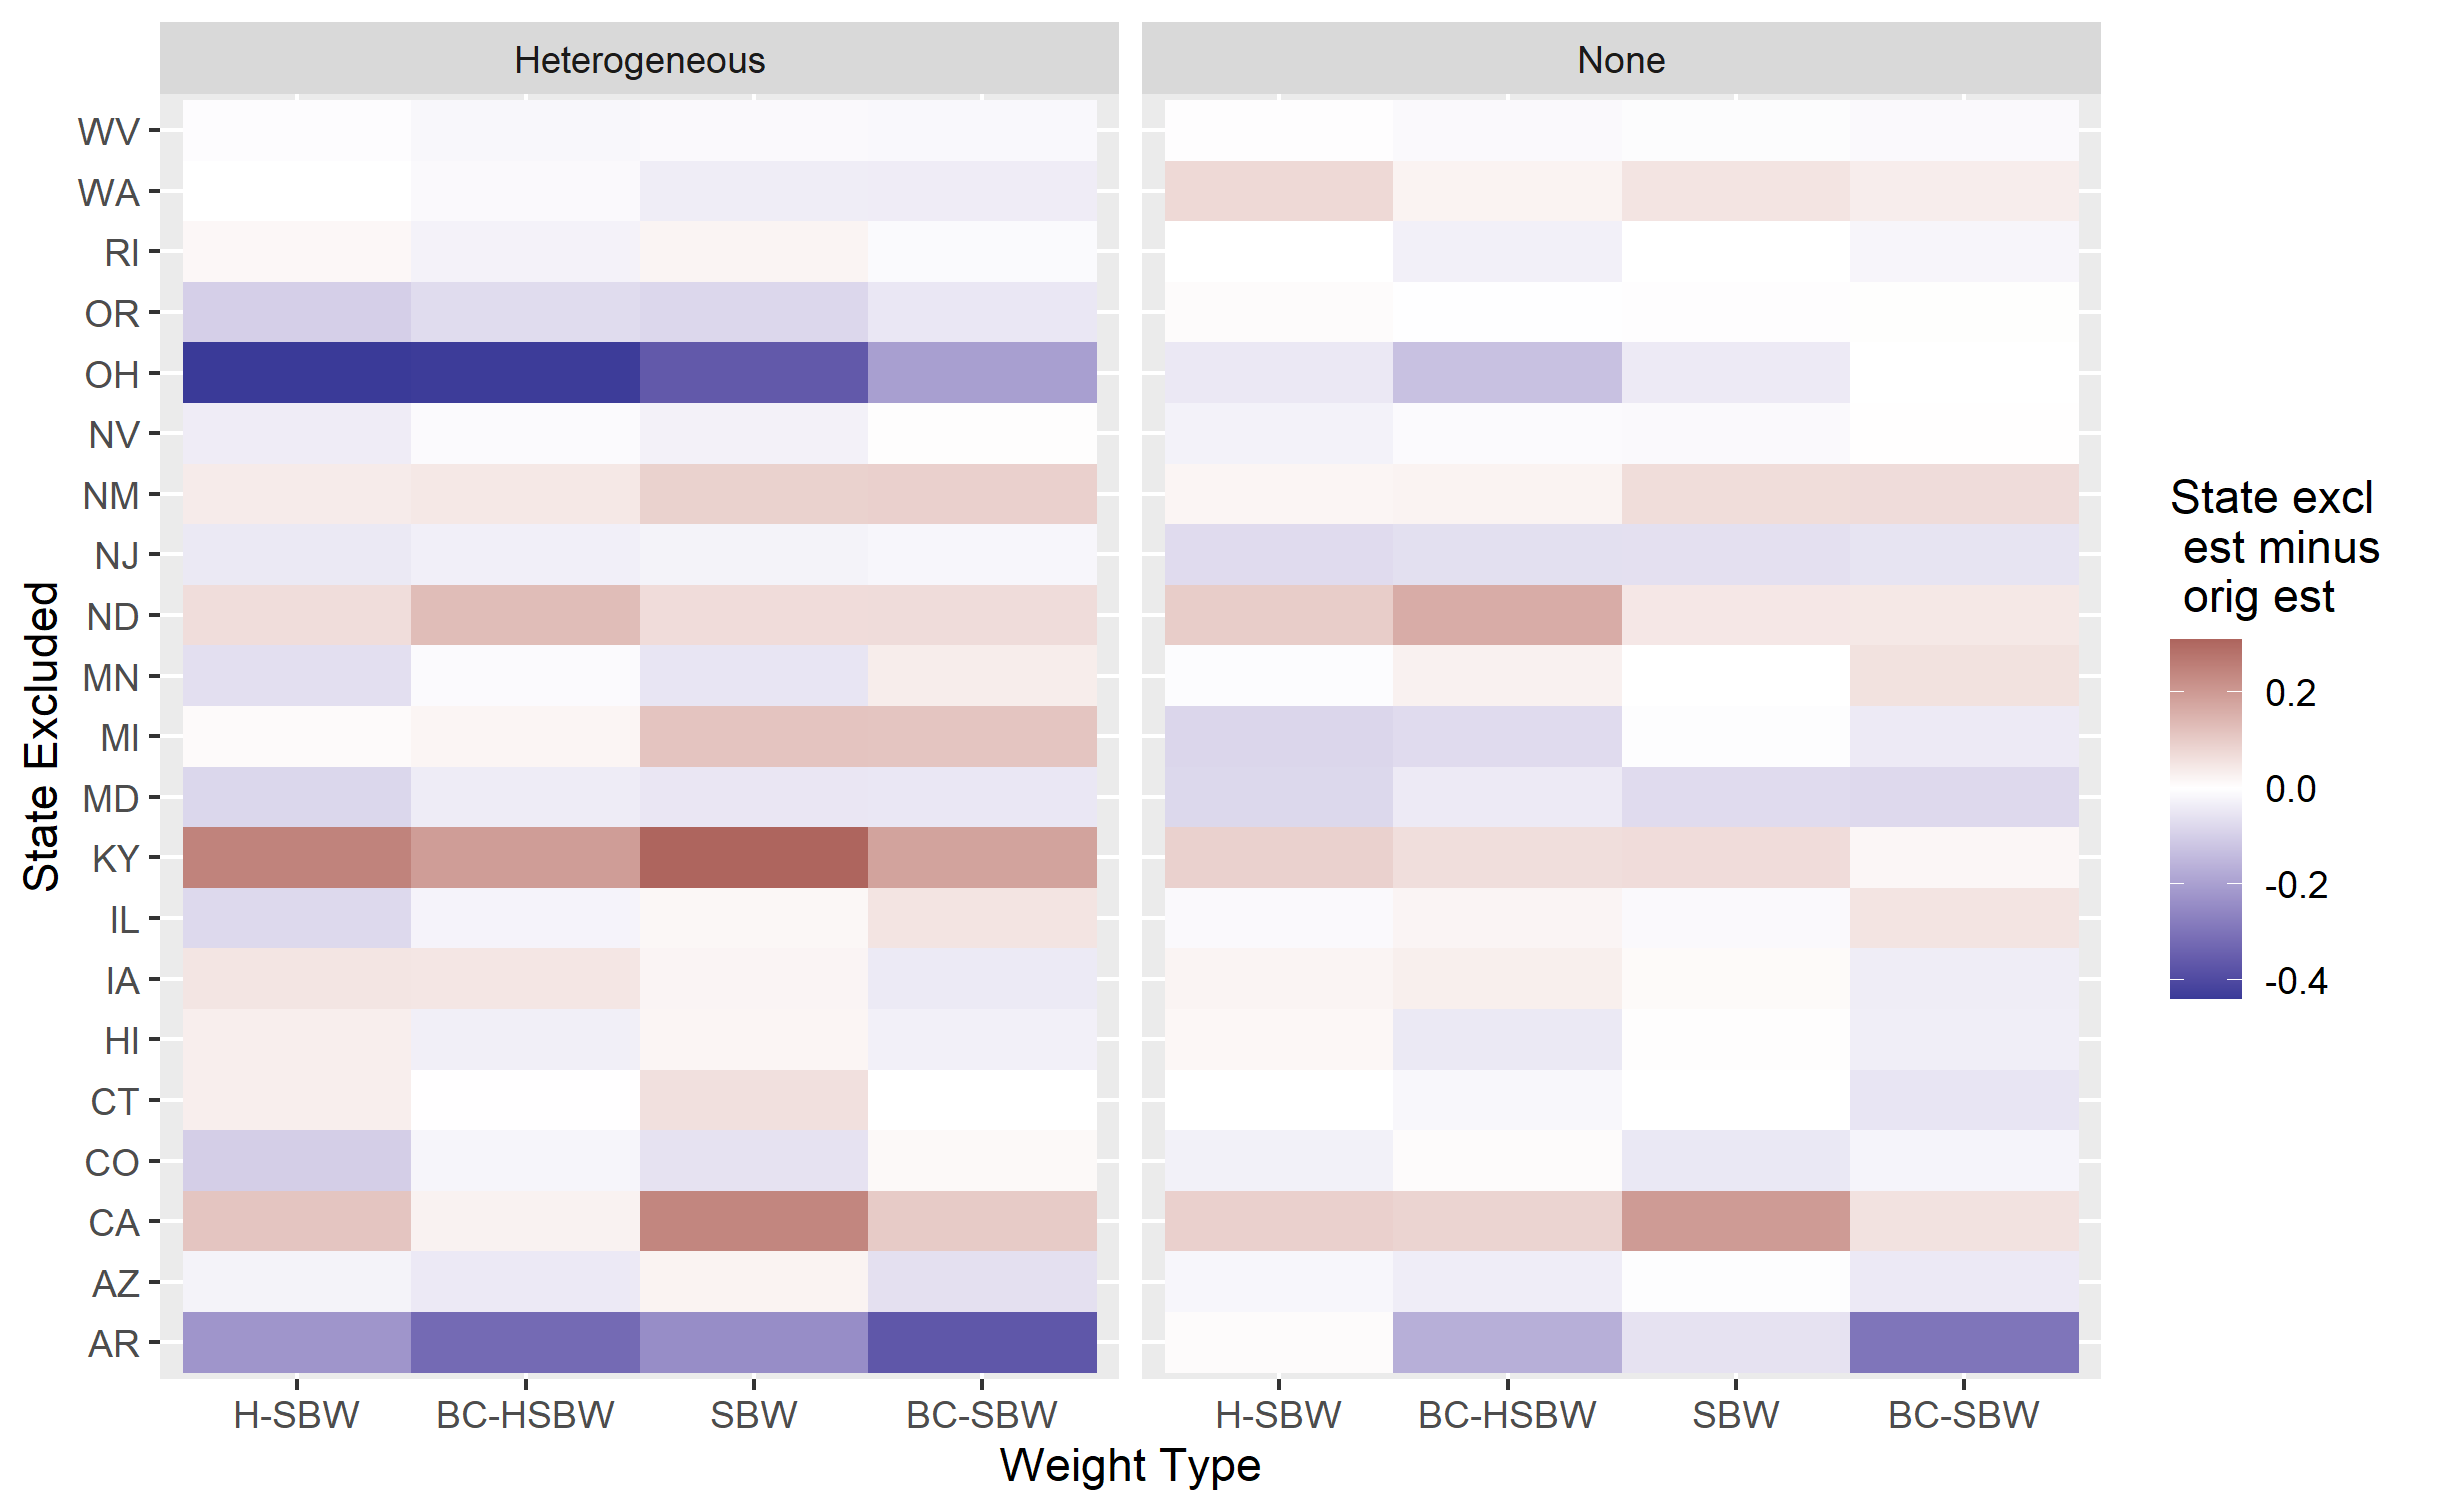
\includegraphics[scale=0.6]{01_Plots/loostate-sensitivityc1-proc-uu-avg.png}
\end{center}
\subcaption{Colors reflect the magnitude of the difference in the estimates when subtracting the original estimate from the estimate that excludes the specified state. The values in the right panel are on the unadjusted data.}
\end{figure}

\clearpage
